\chapter{PicnicAuth}

\section{Architektura projektu}
Projekt składa się z trzech komponentów: serwera w architekturze REST (Representational state transfer) API, 
informacyjnej strony internetowej oraz bibliotek klienckich. Komponenty te są od siebie niezależne, dzięki czemu 
łatwa jest rozbudowa projektu, jak również wersjonowanie każdego z nich.

\subsection{REST API}
Pierwszym z nich jest serwer implementujący logikę aplikacji. 
Jest on stworzony w technologii \textit{ASP.NET Web API 2} w języku programowania \textit{C\#}. \\
Przy jego tworzeniu zostały zachowane zasady architektury REST, co pozwala na łatwą i sprawną integracją
platform klienckim, niezależnie od użytej technologii. \\ \\
Zasoby udostępniane przez REST API to:
\begin{itemize}
	\item \textit{[GET] /api/Companies/Me/AuthUsers} \\
		Zwraca listę użytkowników dla aktualnie zalogowanego podmiotu.
	\item \textit{[POST] /api/AuthUsers} \\
		Tworzy nowego użytkownika i dodaje go do kolekcji użytkowników zalogowanego podmiotu.
		W odpowiedzi zwracany jest sekret stworzonego użytkownika, jak również link 
		do kodu QR kompatybilnego z aplikacjami mobilnymi.
	\item \textit{[PATCH] /api/AuthUsers/{userId}/secret} \\
		Generuje nowy sekret dla użytkownika o podanym \textit{userdId}.
	\item \textit{[GET] /api/Companies/Me} \\ 
		Zwraca dane zalogowanego podmiotu, takie jak login, adres poczty elektronicznej oraz unikalny identyfikator.
	\item \textit{[POST] /api/Companies} \\
		Tworzy nowe konto podmiotu. 
	\item \textit{[GET] /api/AuthUsers/{userId}/hotp} \\
		Zwraca hasło jednorazowe typu \textit{HOTP} dla użytkownika o podanym \textit{userId}.
	\item \textit{[GET] /api/AuthUsers/{userId}/totp} \\
		Zwraca hasło jednorazowe typu \textit{TOTP} dla użytkownika o podanym \textit{userId}.
	\item \textit{[GET] /api/AuthUsers/{userId}/hotp/{hotp}} \\
		Zwraca wynik weryfikacji podanego hasła jednorazowego typu \textit{HOTP}
	\item \textit{[GET] /api/AuthUsers/{userId}/totp/{totp}} \\
		Zwraca wynik weryfikacji podanego hasła jednorazowego typu \textit{TOTP}
	\item \textit{[POST] /api/tokens}
		Zwraca klucz API, który służy do uwierzytelnienia podmiotu. (Równoznaczne z logowaniem,
		zgodnym ze standardem \textit{OAuth}.)
\end{itemize}
Zasoby na których operuje API są w formacie JSON (JavaScript Object Notation), zarówno przy metodach, które
przyjmują dane, jak i tych, które zwracają dane. \\
Za pomocą pakietu \textit{Swashbuckle} skonfigurowana została automatyczna generacja dokumentacji API
na podstawie publicznie wystawionych kontrolerów. 
Oprócz podstawowych informacji o metodach znajdujących się w kontrolerach, takich jak nazwy czy typy parametrów, 
w~dokumentacji umieszczane są także komentarze, którymi opisana jest dana metoda. Oprócz funkcji informacyjnej, 
wygenerowana dokumentacja pozwala na wygodne testy każdej z metod. 
Końcowy efekt wygenerowanej dokumentacji przedstawiony jest na Rysunku \ref{swagger}. \\
Aplikacja przeznaczona jest do działania na serwerze \textit{IIS (Internet Information Service)} w~wersji~7.
\begin{figure}[t]
    \centering
	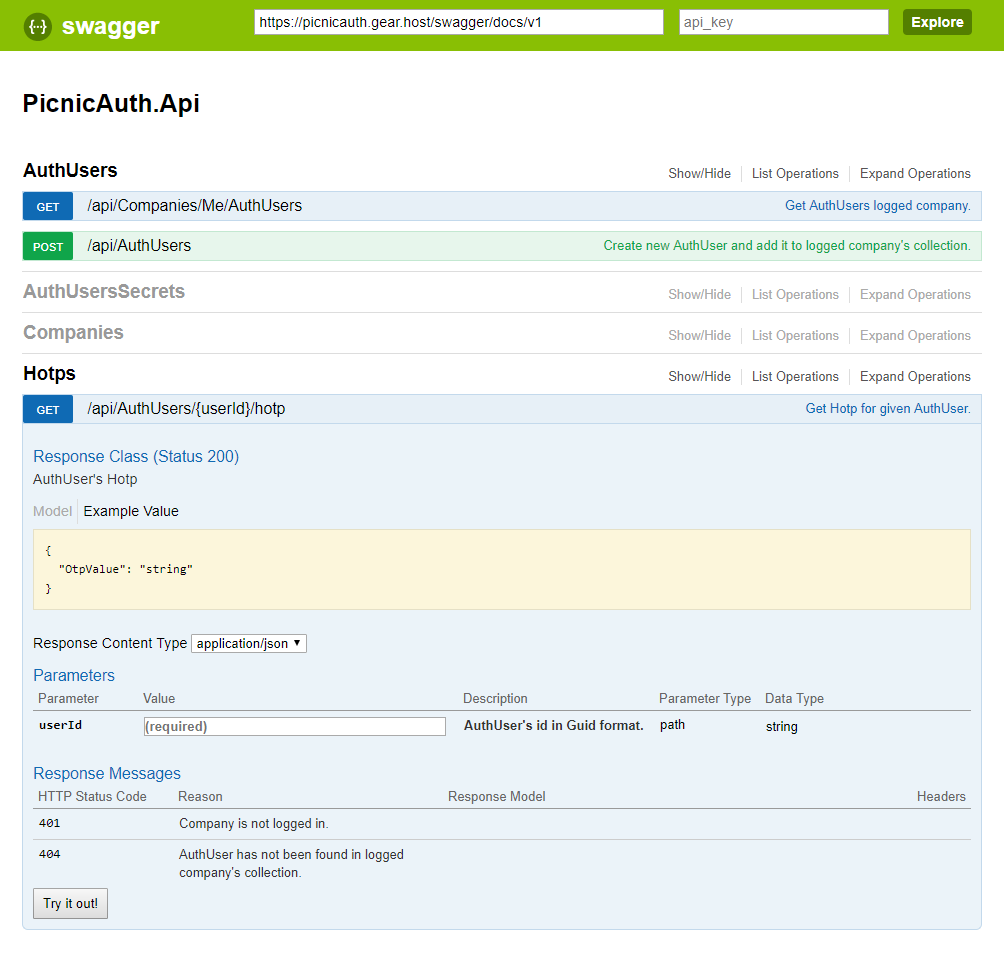
\includegraphics[width=\textwidth]{content/images/swagger}
    \caption{Interaktywna dokumentacja API.}
    \label{swagger}
\end{figure}

\subsection{Frontend}
Strona internetowa projektu (Rysunek \ref{front-home}) stworzona została w technologii \textit{Angular} w wersji~5 w konwencji 
\textit{Single Page Application}. Znajduje się na niej instrukcja użycie projektu jak również informacje
o aktualnej liczbie dostępnych bibliotek. Zawiera ona także przydatne odnośniki do repozytoriów, w których
znajduje się kod źródłowy oraz do strony na której znajduje się dokumentacja API. \\
Dodatkowymi funkcjonalnościami jakie oferuje strona jest stworzenie nowego konta dla podmiotu 
(przedstawione na Rysunku \ref{front-create}), jak również uzyskanie klucza API, 
umożliwiającego użycie bibliotek klienckich.
\begin{figure}[t]
    \centering
	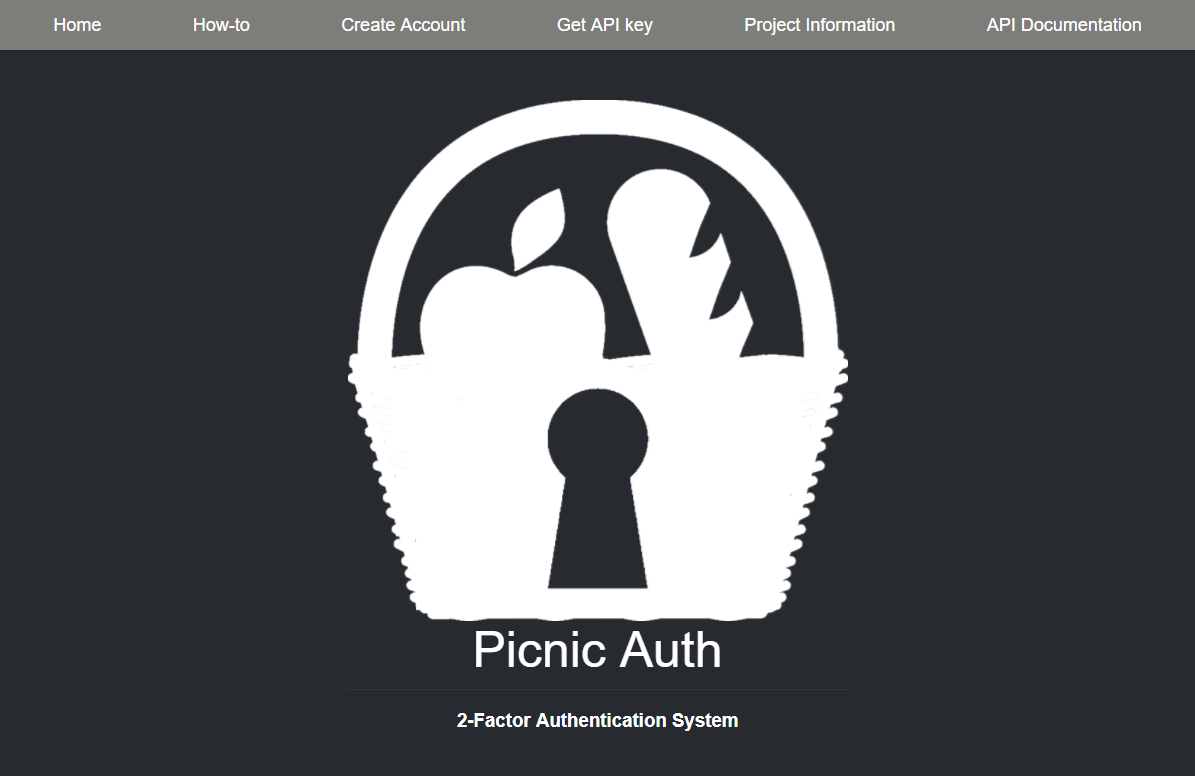
\includegraphics[width=\textwidth]{content/images/front-home}
    \caption{Informacyjna strona internetowa projektu.}
    \label{front-home}
\end{figure}
\begin{figure}[t]
    \centering
	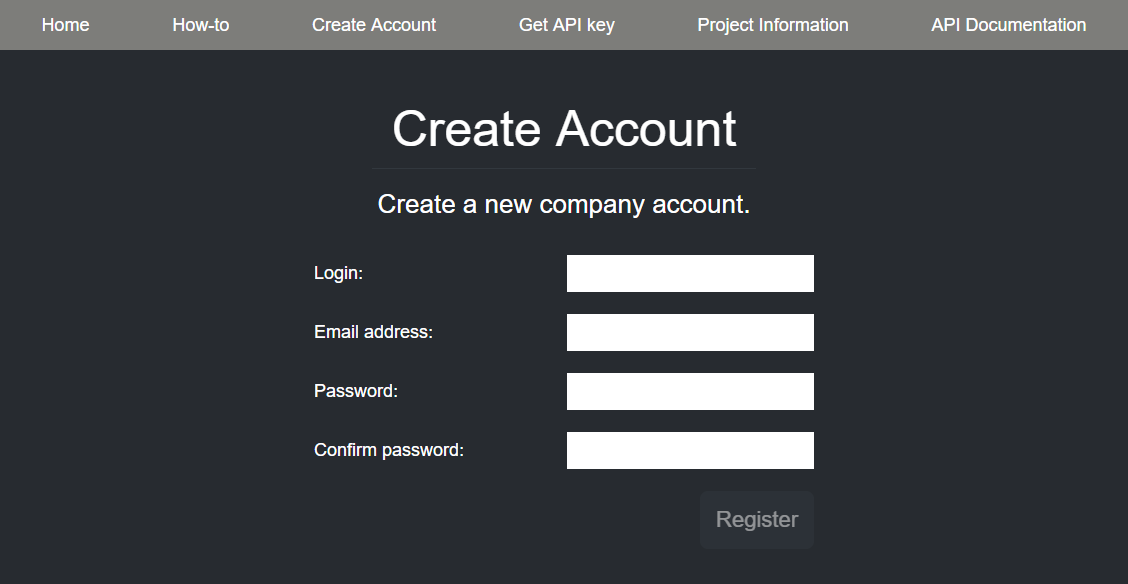
\includegraphics[width=\textwidth]{content/images/front-create}
    \caption{Tworzenie konta podmiotu.}
    \label{front-create}
\end{figure}

\subsection{Biblioteki klienckie}
W celu ułatwienia integracji z serwerem zaimplementowane zostały biblioteki klienckie.
Umożliwiają one w prosty sposób użycie funkcjonalności serwera bez konieczności 
studiowania dokumentacji i pisania kodu odpowiedzialnego za integrację. \\
Przykładowo biblioteka w języku C\# udostępnia klasę \textit{PicnicAuthClient}, posiadająca metody:
\begin{itemize}
	\item Login
	\item GetAuthUsers
	\item AddAuthUser
	\item GenereteNewSecret
	\item GetLoggedCompany
	\item AddCompany
	\item GetHotpForAuthUser
	\item ValidateHotpForAuthUser
	\item GetTotpForAuthUser
	\item ValidateTotpForAuthUser
\end{itemize}
Na chwilę obecną gotowe do użycia są biblioteki w następujących technologiach:
\begin{enumerate}
	\item C\#
	\item Visual Basic
	\item TypeScript
	\item Python 3.6
	\item Python 2.7
	\item Ruby
\end{enumerate}

\section{Dostarczanie sekretu na urządzenie mobilne}
\begin{figure}[t]
    \centering
	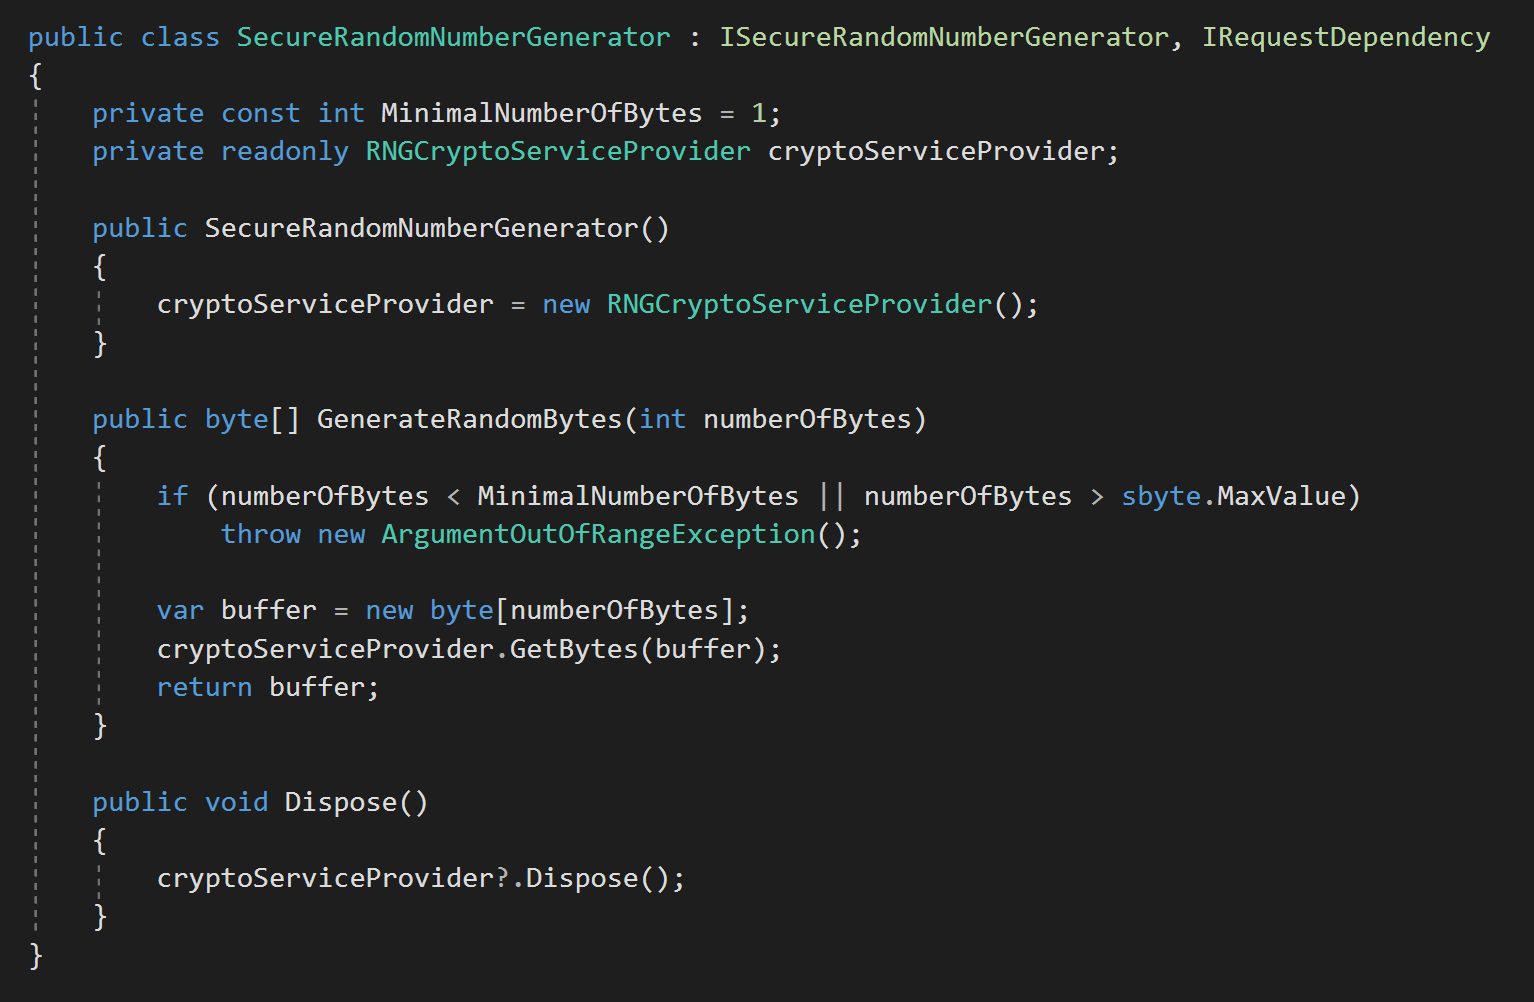
\includegraphics[width=\textwidth]{content/images/code-srng}
    \caption{Klasa zwracająca kryptograficznie bezpiecznie pseudolosowe dane.}
    \label{code-srng}
\end{figure}
\begin{figure}[t]
    \centering
	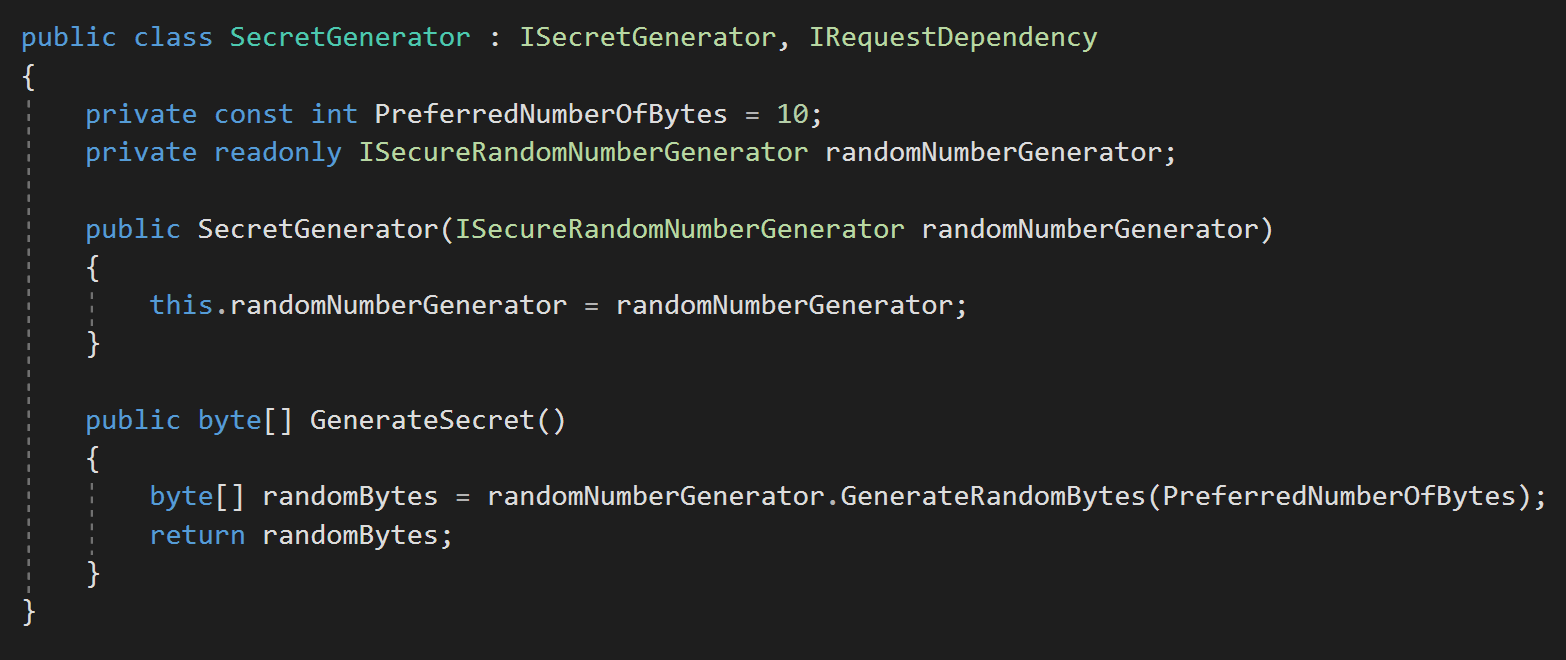
\includegraphics[width=\textwidth]{content/images/code-secretgenerator}
    \caption{Klasa generująca sekret użytkownika.}
    \label{code-secretgenerator}
\end{figure}
\begin{figure}[t]
    \centering
	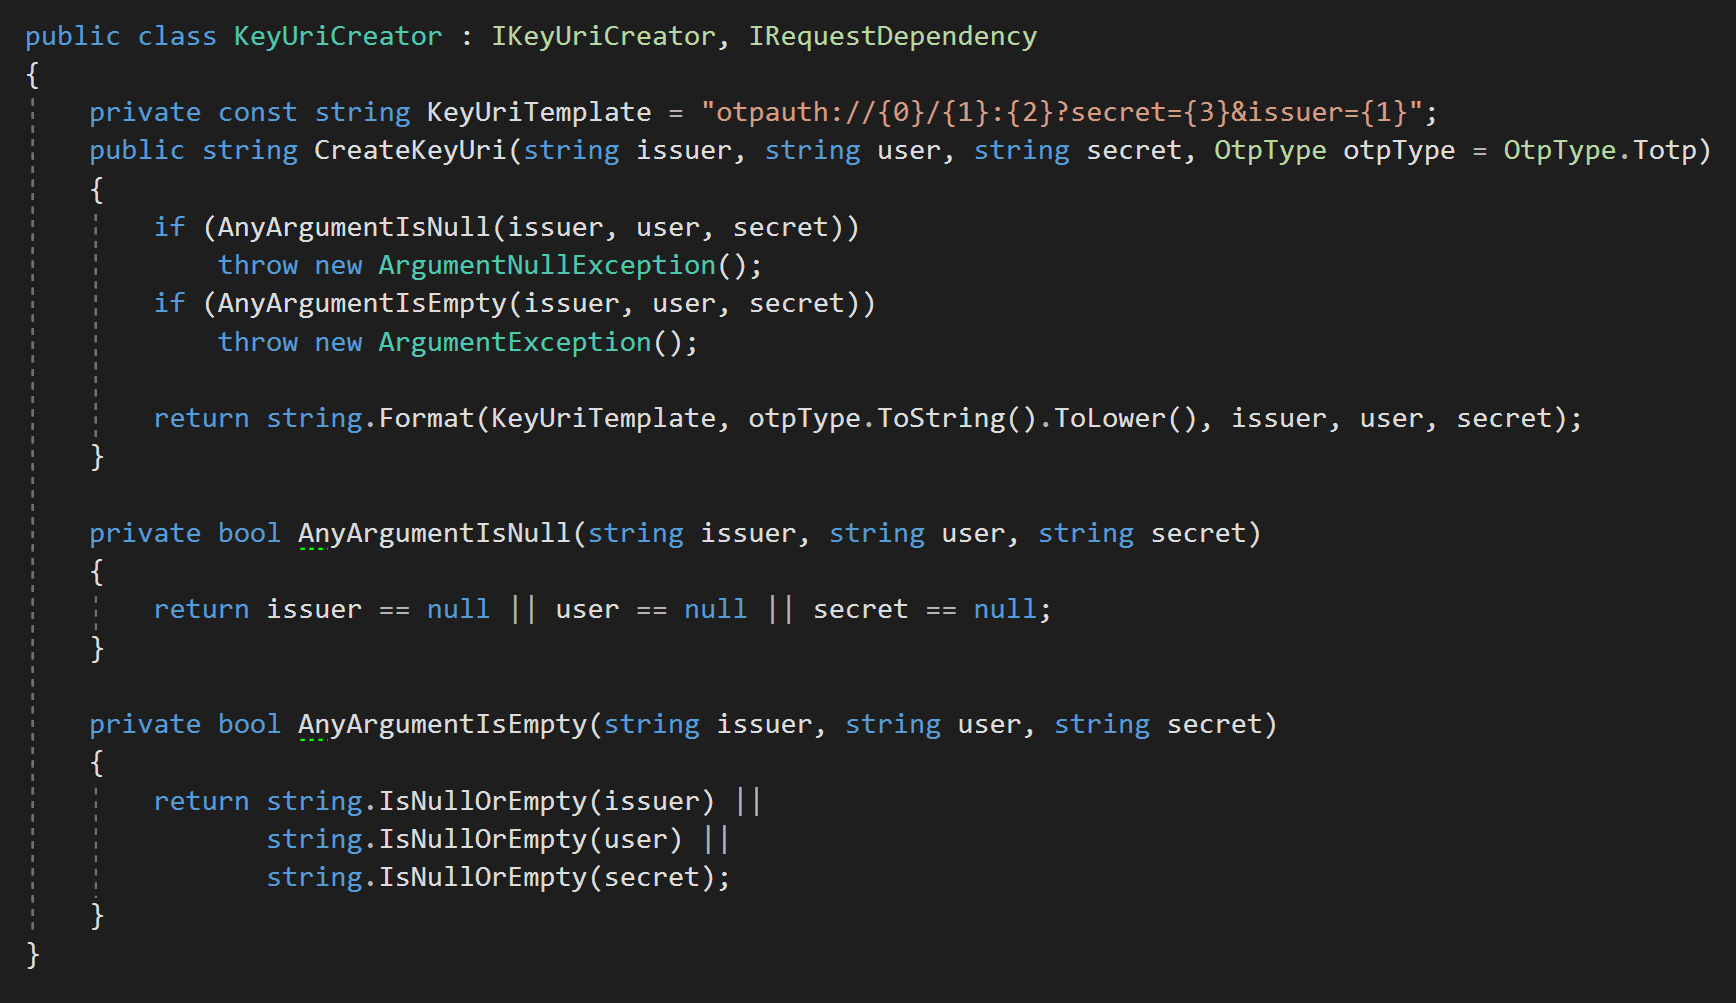
\includegraphics[width=\textwidth]{content/images/code-keyuri}
    \caption{Klasa generująca KeyUri.}
    \label{code-keyuri}
\end{figure}
\section{Generowanie OTP po stronie serwera}
\begin{figure}[t]
    \centering
	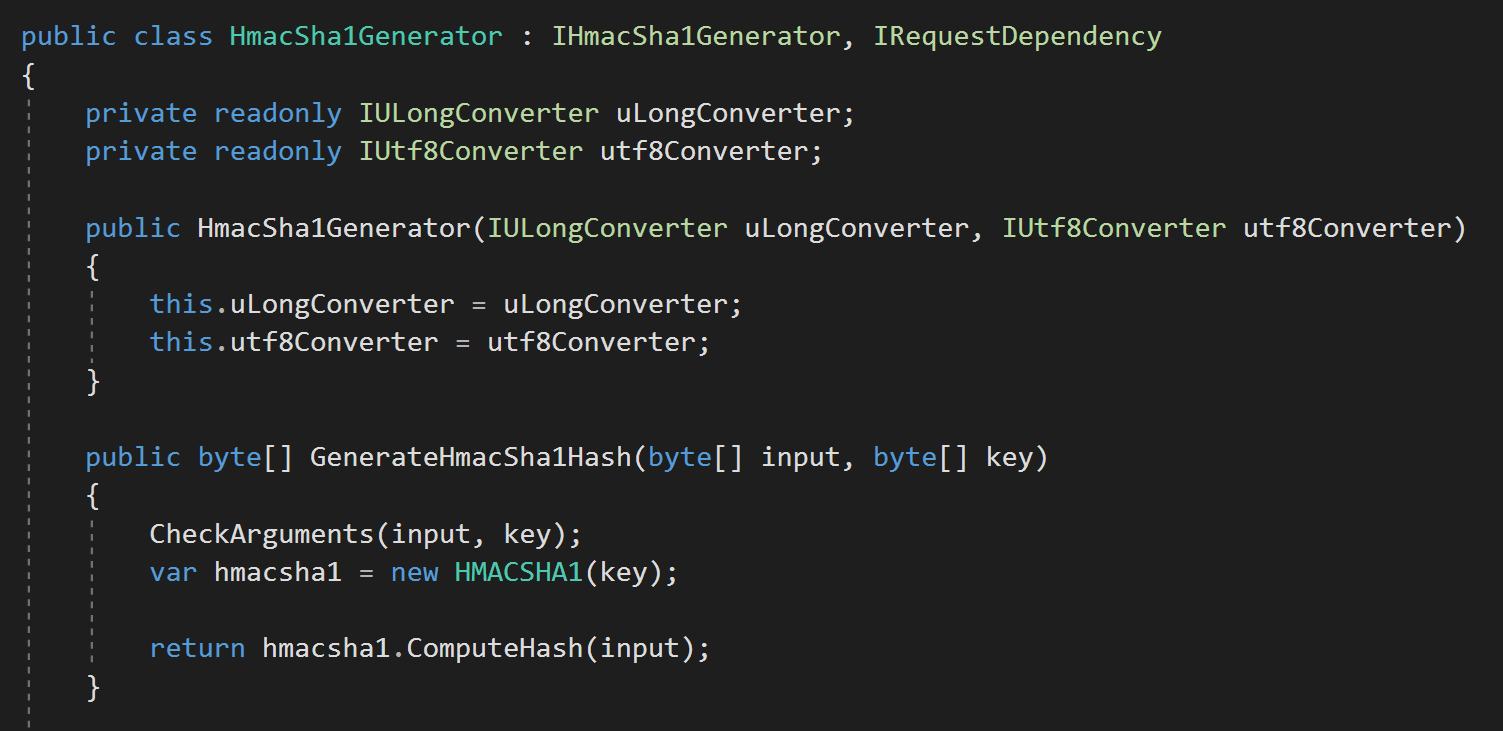
\includegraphics[width=\textwidth]{content/images/code-hmac}
    \caption{Klasa generująca HMAC.}
    \label{code-hmac}
\end{figure}
\begin{figure}[t]
    \centering
	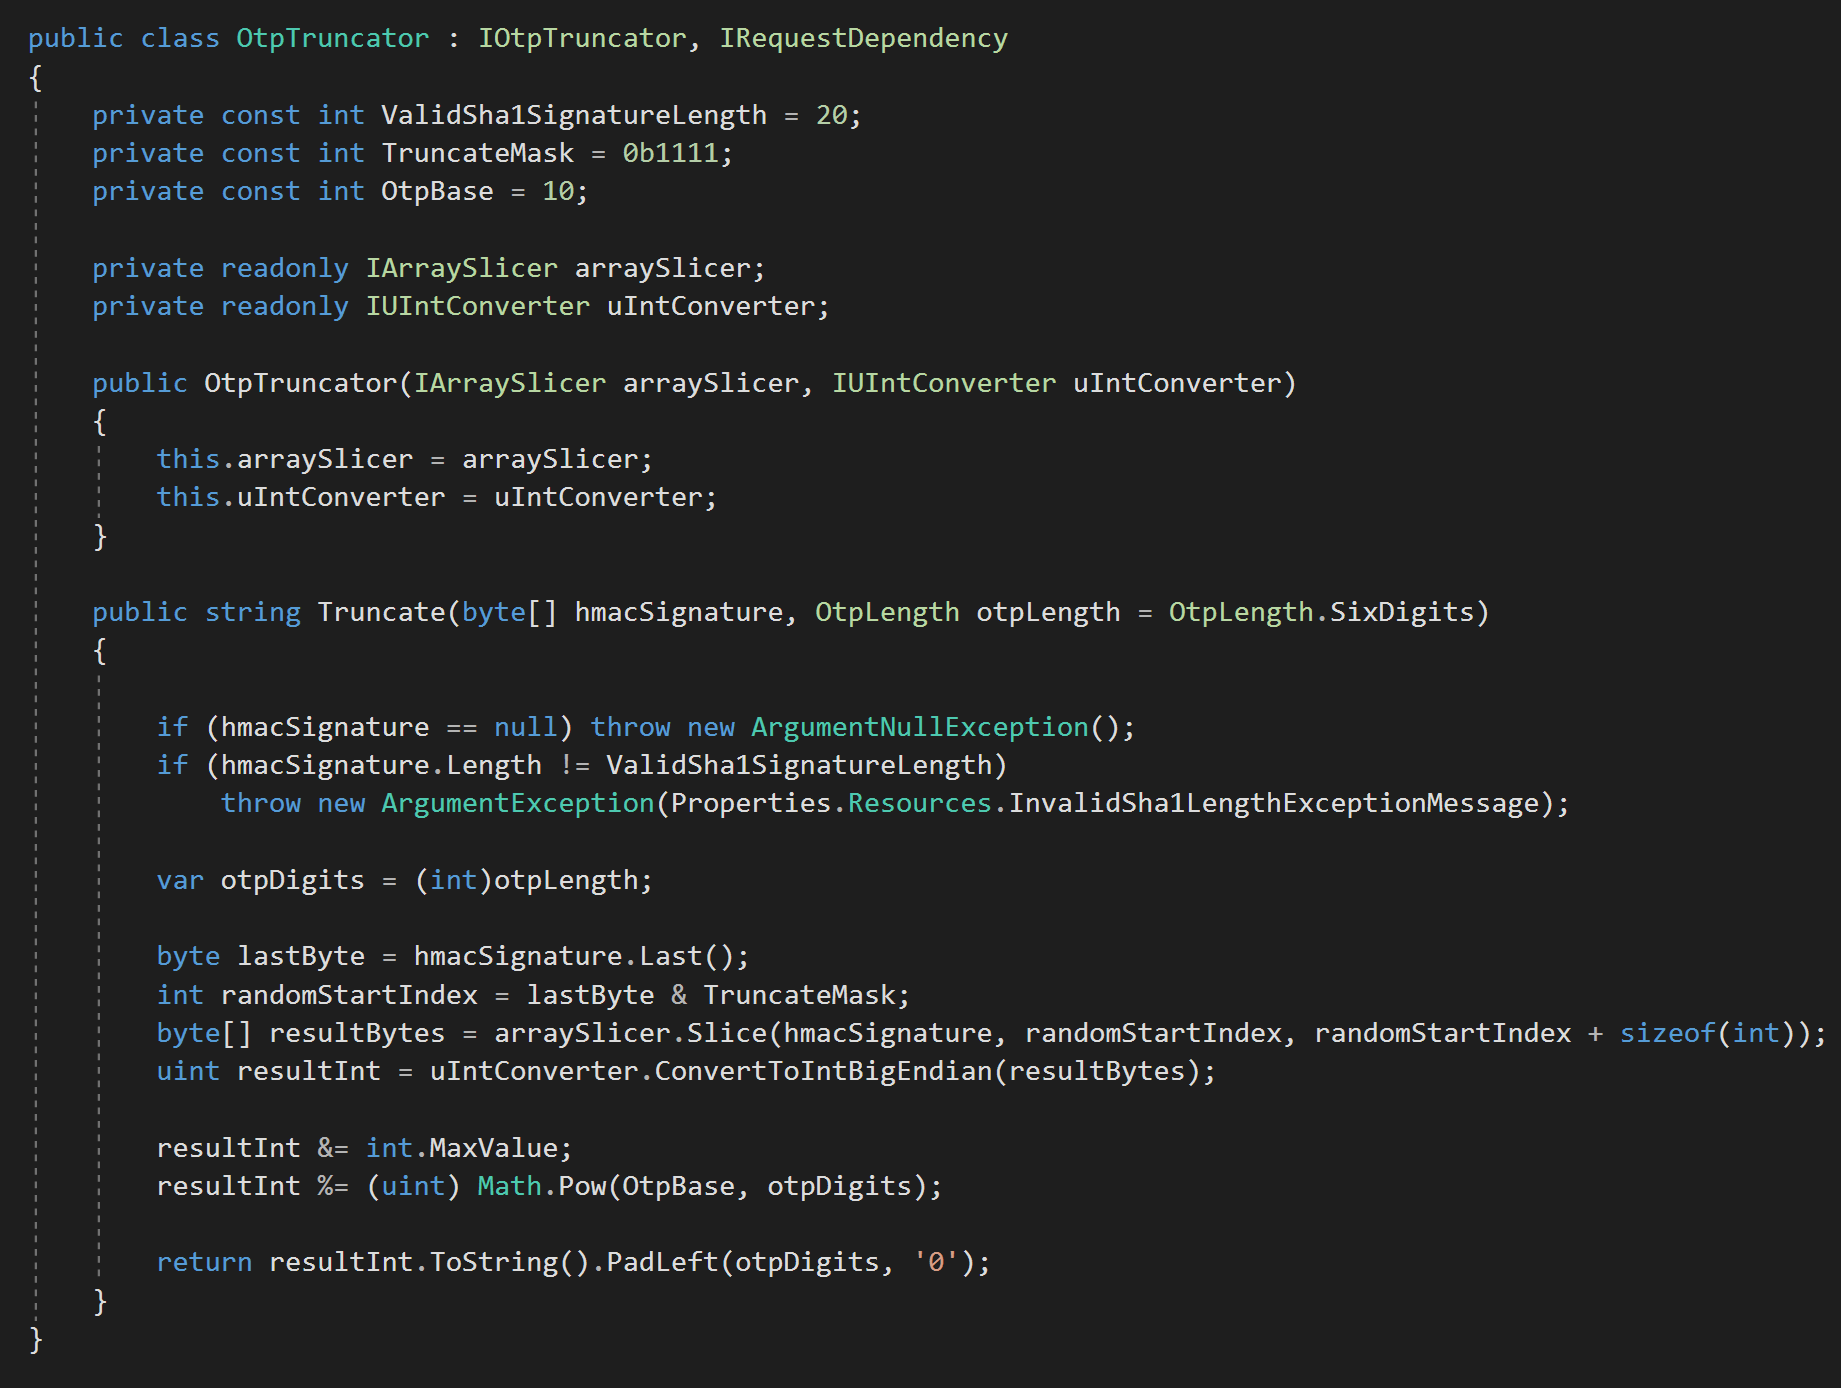
\includegraphics[width=\textwidth]{content/images/code-truncator}
    \caption{Klasa odpowiedzialna za przycięcie wyniku HMAC do postaci hasła.}
    \label{code-truncator}
\end{figure}
\begin{figure}[t]
    \centering
	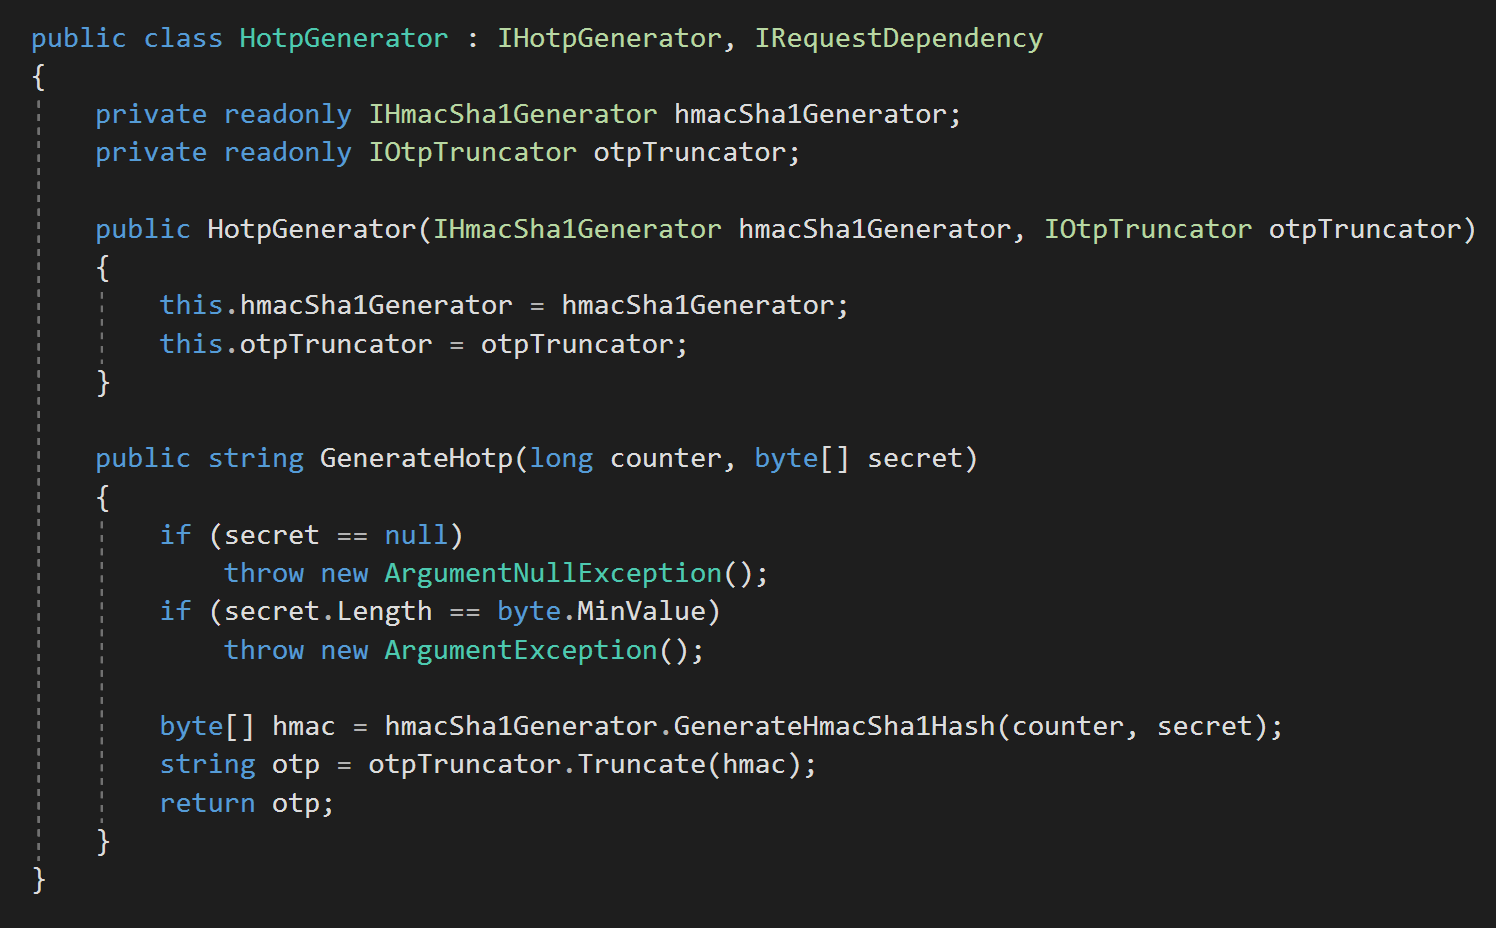
\includegraphics[width=\textwidth]{content/images/code-hotpgenerator}
    \caption{Klasa generująca hasło jednorazowe oparte o licznik.}
    \label{code-hotp}
\end{figure}
\begin{figure}[t]
    \centering
	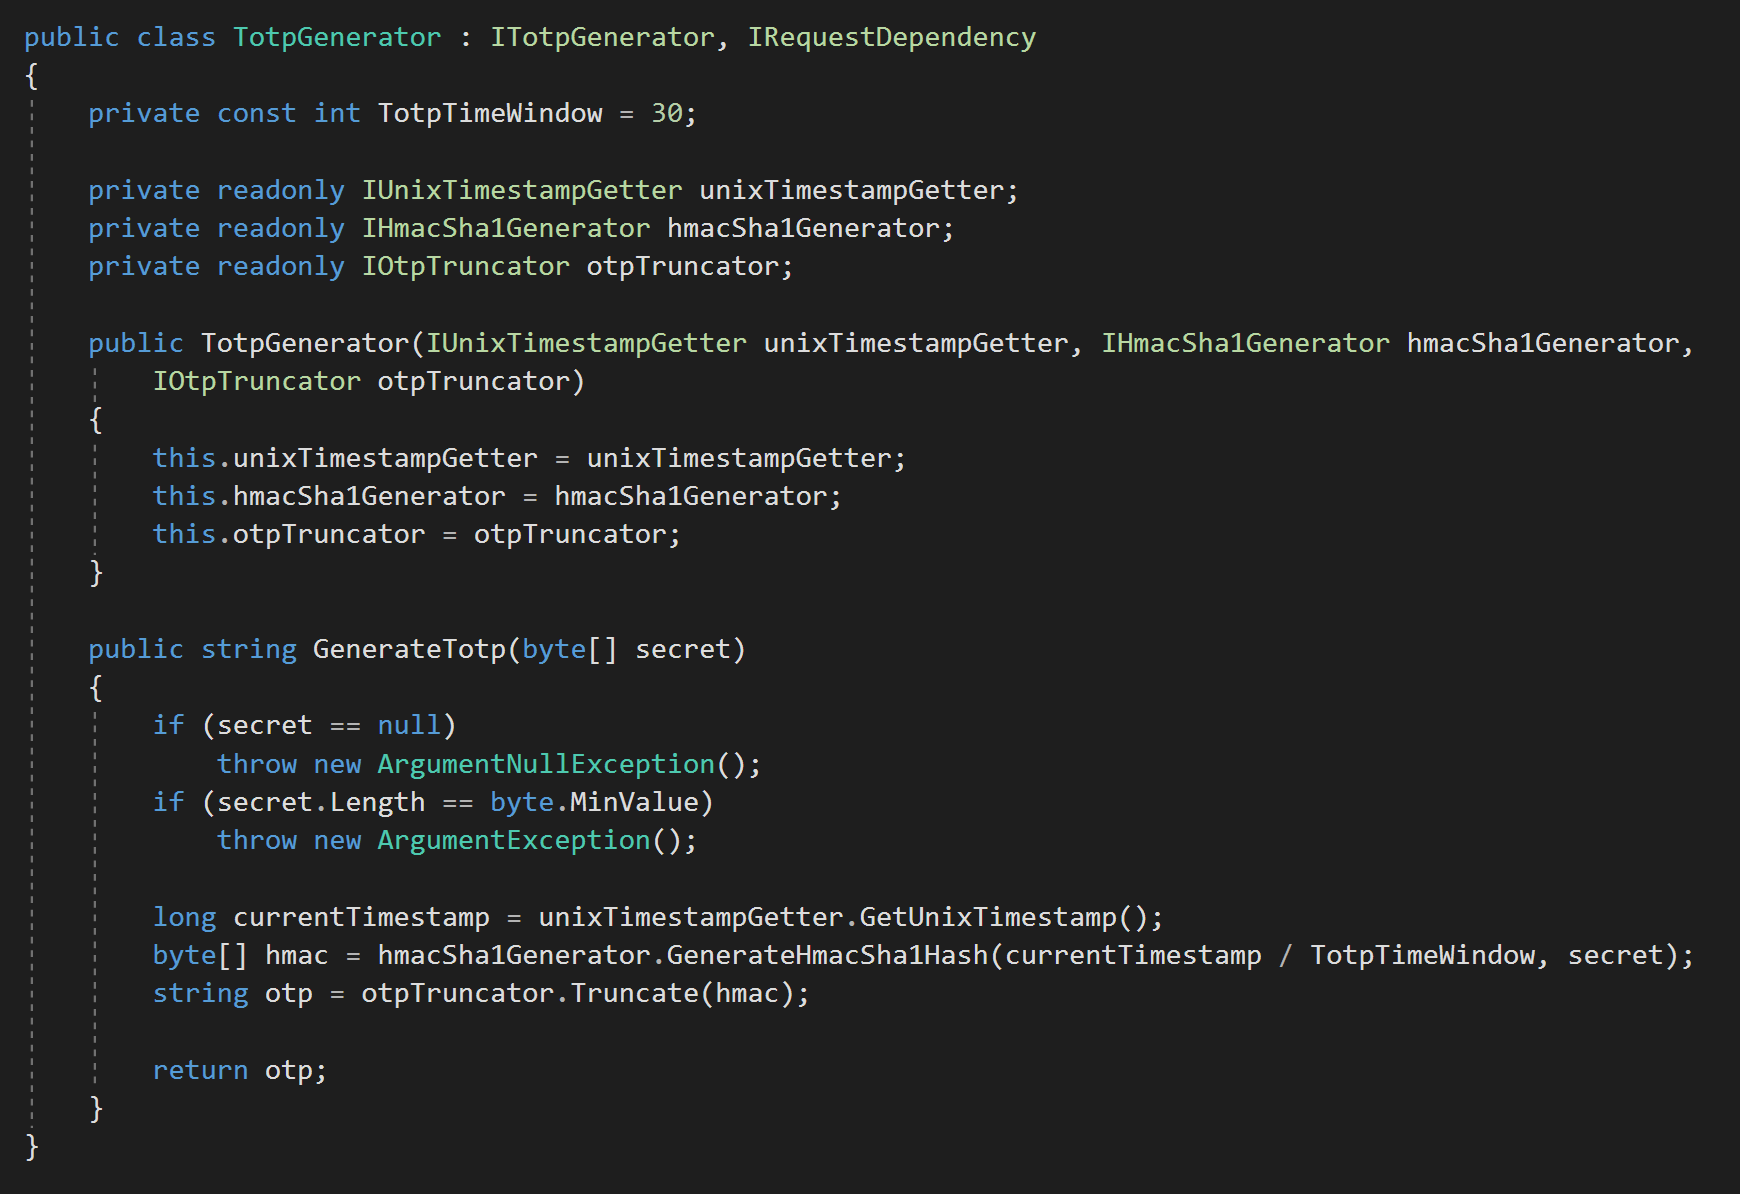
\includegraphics[width=\textwidth]{content/images/code-totpgenerator}
    \caption{Klasa generująca hasło jednorazowe oparte o czas.}
    \label{code-totp}
\end{figure}
\section{Generowanie OTP po stronie użytkownika}
\section{Przechowywanie sekretu użytkownika}
\begin{figure}[t]
    \centering
	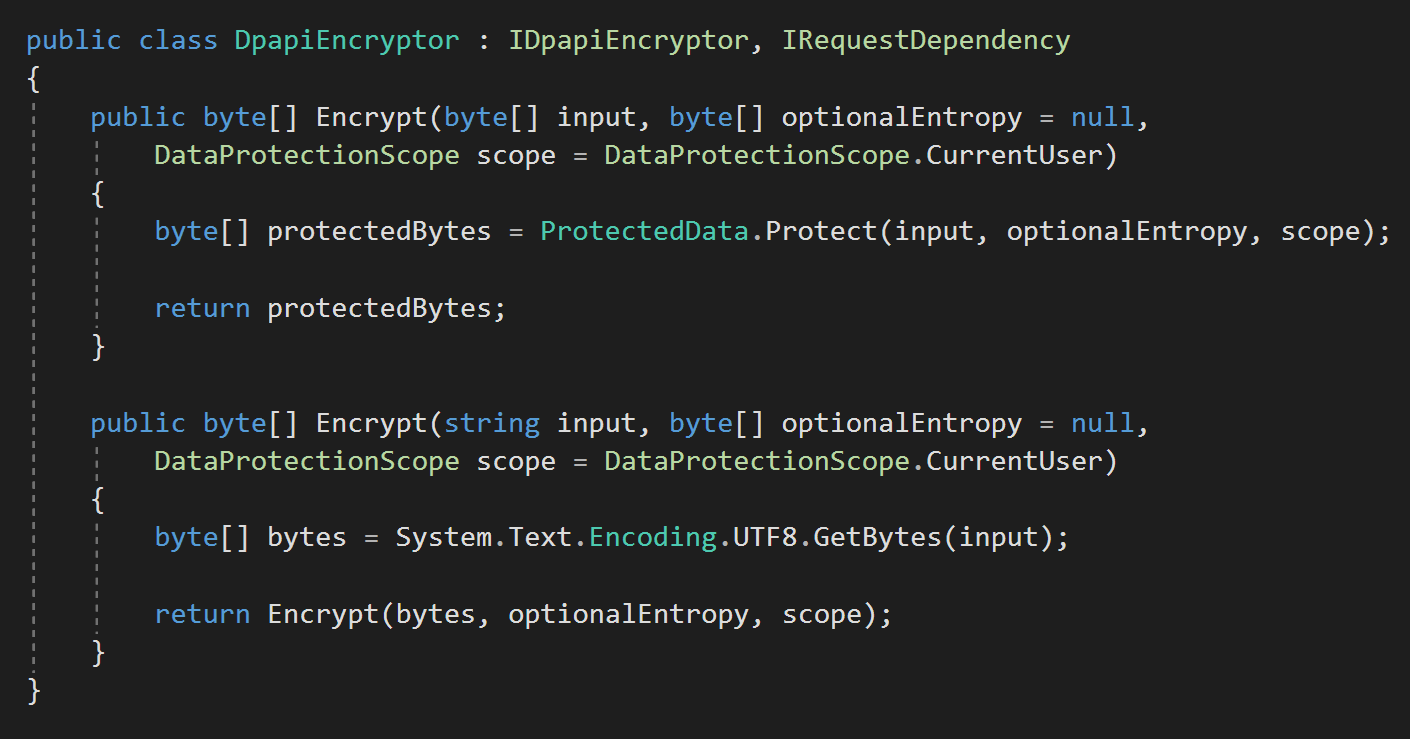
\includegraphics[width=\textwidth]{content/images/code-encrypt}
    \caption{Klasa odpowiedzialna za szyfrowanie.}
    \label{code-encrypt}
\end{figure}
\begin{figure}[t]
    \centering
	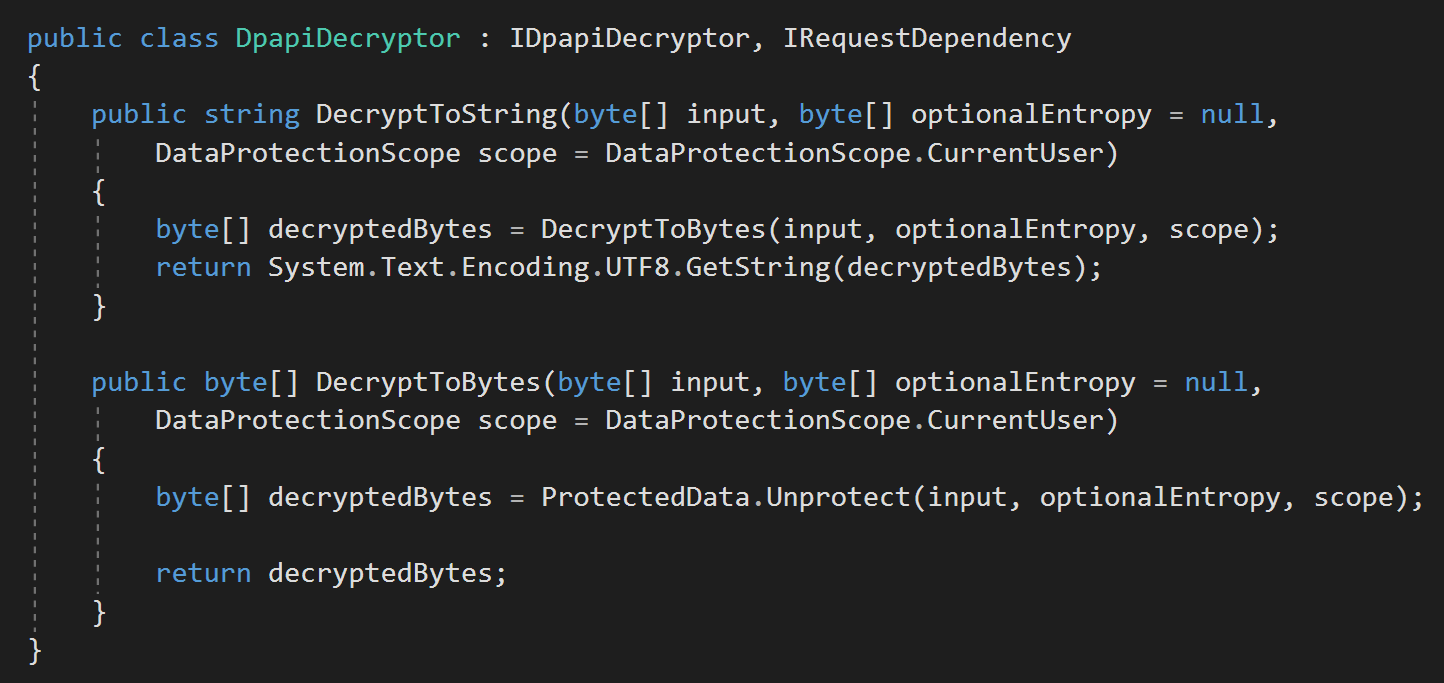
\includegraphics[width=\textwidth]{content/images/code-decrypt}
    \caption{Klasa odpowiedzialna za deszyfrowanie.}
    \label{code-decrypt}
\end{figure}
\section{Przykład użycia projektu}
\section{Planowane ulepszenia}

